\documentclass{article}
\usepackage[utf8]{inputenc}
\usepackage{amsmath, amssymb}
\usepackage{float}
\usepackage{hyperref}
\usepackage{natbib}
\usepackage{booktabs}
\usepackage{graphicx}
\usepackage{algorithm}
\usepackage{algpseudocode}

\title{Sentiment Analysis on Twitter Data}
\author{John Doe}
\date{\today}

\begin{document}
\maketitle

\section{Introduction}
Lorem ipsum dolor sit amet, consetetur sadipscing elitr, sed diam nonumy eirmod tempor invidunt ut labore et dolore magna aliquyam erat, sed diam voluptua. At vero eos et accusam et justo duo dolores et ea rebum. Stet clita kasd gubergren, no sea takimata sanctus est Lorem ipsum dolor sit amet. Lorem ipsum dolor sit amet, consetetur sadipscing elitr, sed diam nonumy eirmod tempor invidunt ut labore et dolore magna aliquyam erat, sed diam voluptua. At vero eos et accusam et justo duo dolores et ea rebum.

Some related work would be Word2Vec~\cite{Word2Vec} or BERT~\cite{BERT}.


\section{Approach}
Ut wisi enim ad minim veniam, quis nostrud exerci tation ullamcorper suscipit lobortis nisl ut aliquip ex ea commodo consequat. Duis autem vel eum iriure dolor in hendrerit in vulputate velit esse molestie consequat, vel illum dolore eu feugiat nulla facilisis at vero eros et accumsan et iusto odio dignissim qui blandit praesent luptatum zzril delenit augue duis dolore te feugait nulla facilisi:

\begin{align}
    \cfrac{1}{m}\sum_{i=1}^m(y_i - f(x_i)^2)
    \label{eq:equation1}
\end{align}

Equation~\ref{eq:equation1} tempor cum soluta nobis eleifend option congue nihil imperdiet doming id quod mazim placerat facer possim assum. Lorem ipsum dolor sit amet, consectetuer adipiscing elit, sed diam nonummy nibh euismod tincidunt ut laoreet dolore magna aliquam erat volutpat. Ut wisi enim ad minim veniam, quis nostrud exerci tation ullamcorper suscipit lobortis nisl ut aliquip ex ea commodo consequat.

\begin{algorithm}[h]
    \begin{algorithmic}
        \State $f_0 \gets 1$
        \State $f_1 \gets 1$
        \For{$i=2\dots,n$}
        \State $f_i=f_{i-1}+f_{i-2}$
        \EndFor\\
        \Return $f_n$
    \end{algorithmic}
    \caption{Pseudocode}
    \label{alg:cap}
\end{algorithm}

Algorithm~\ref{alg:cap} autem vel eum iriure dolor in hendrerit in vulputate velit esse molestie consequat, vel illum dolore eu feugiat nulla facilisis.


\section{Experiments}
Duis autem vel eum iriure dolor in hendrerit in vulputate velit esse molestie consequat, vel illum dolore eu feugiat nulla facilisis at vero eros et accumsan et iusto odio dignissim qui blandit praesent luptatum zzril delenit augue duis dolore te feugait nulla facilisi. Lorem ipsum dolor sit amet, consectetuer adipiscing elit, sed diam nonummy nibh euismod tincidunt ut laoreet dolore magna aliquam erat volutpat.

\begin{figure}[ht]
    \centering
    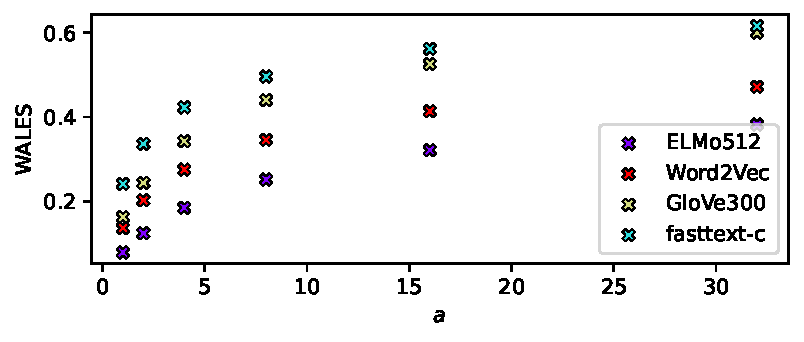
\includegraphics[width=\textwidth]{figures/power.pdf}
    \caption{Some Figure}
    \label{fig:figure1}
\end{figure}

Figure~\ref{fig:figure1} enim ad minim veniam, quis nostrud exerci tation ullamcorper suscipit lobortis nisl ut aliquip ex ea commodo consequat. Duis autem vel eum iriure dolor in hendrerit in vulputate velit esse molestie consequat, vel illum dolore eu feugiat nulla facilisis at vero eros et accumsan et iusto odio dignissim qui blandit praesent luptatum zzril delenit augue duis dolore te feugait nulla facilisi.

\begin{table}[hb]
    \centering
    \begin{tabular}{lll}
        Approach & Score & Time \\
        \toprule
        name1    & 0.45  & 0.10 \\
        name2    & 0.55  & 0.13 \\
        name3    & 0.75  & 0.22
    \end{tabular}
    \caption{Some Table}
    \label{tab:table1}
\end{table}
Table~\ref{tab:table1} liber tempor cum soluta nobis eleifend option congue nihil imperdiet doming id quod mazim placerat facer possim assum. Lorem ipsum dolor sit amet, consectetuer adipiscing elit, sed diam nonummy nibh euismod tincidunt ut laoreet dolore magna aliquam erat volutpat. Ut wisi enim ad minim veniam, quis nostrud exerci tation ullamcorper suscipit lobortis nisl ut aliquip ex ea commodo

\bibliographystyle{plain}
\bibliography{references}
\end{document}
